\documentclass{standalone} 
         \usepackage{graphicx} 
 \usepackage[hang,small,bf]{caption}    % fancy captions
 \usepackage{tikz}	

% TikZ libraries 
\usetikzlibrary{shapes,snakes} 
\usetikzlibrary{backgrounds,fit,decorations.pathreplacing} 
 \usetikzlibrary{shapes,arrows,fit,calc,positioning,automata} 
\newcommand{\ket}[1]{\ensuremath{\left|#1\right\rangle}} % Dirac Kets 
\begin{document} 
    %\begin{figure} 
    %\centerline{ 
        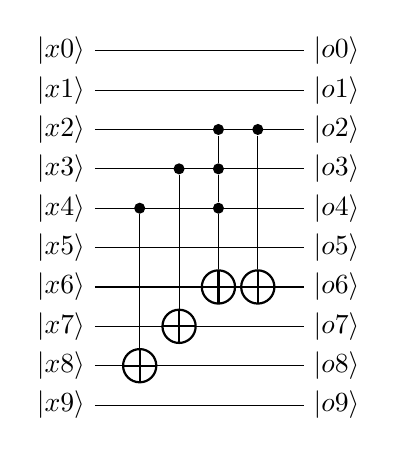
\begin{tikzpicture}[] 
            \tikzset{oplus/.style={path picture={% 
            \draw[black] 
            (path picture bounding box.south) -- (path picture bounding box.north) 
            (path picture bounding box.west) -- (path picture bounding box.east);
            }}}
             \tikzstyle{operator} = [draw,fill=white,minimum size=1.5em] 
             \tikzstyle{phase} = [fill,shape=circle,minimum size=4pt,inner sep=0pt]
             \tikzstyle{surround} = [fill=blue!10,thick,draw=black,rounded corners=2mm]
             \tikzstyle{swap} = [draw,fill,shape=cross out,minimum size=5pt,inner sep=0pt]
             \tikzstyle{cnot} = [oplus,draw,thick,circle,minimum size = 12pt]		% Qubit
		\node at (0,-0.0)(q0_0) {\ket{x0}};
		\node at (0,-0.5)(q0_1) {\ket{x1}};
		\node at (0,-1.0)(q0_2) {\ket{x2}};
		\node at (0,-1.5)(q0_3) {\ket{x3}};
		\node at (0,-2.0)(q0_4) {\ket{x4}};
		\node at (0,-2.5)(q0_5) {\ket{x5}};
		\node at (0,-3.0)(q0_6) {\ket{x6}};
		\node at (0,-3.5)(q0_7) {\ket{x7}};
		\node at (0,-4.0)(q0_8) {\ket{x8}};
		\node at (0,-4.5)(q0_9) {\ket{x9}};
		% Gate 1
		\node[phase] (q1_4) at (1.0,-2.0) {} edge [-] (q0_4);
		\node[cnot] (q1_8) at (1.0,-4.0) {} edge [-] (q0_8);
		\draw[-] (q1_4)  -- (q1_8);
		% Gate 2
		\node[phase] (q2_3) at (1.5,-1.5) {} edge [-] (q0_3);
		\node[cnot] (q2_7) at (1.5,-3.5) {} edge [-] (q0_7);
		\draw[-] (q2_3)  -- (q2_7);
		% Gate 3
		\node[phase] (q3_2) at (2.0,-1.0) {} edge [-] (q0_2);
		\node[phase] (q3_3) at (2.0,-1.5) {} edge [-] (q2_3);
		\node[phase] (q3_4) at (2.0,-2.0) {} edge [-] (q1_4);
		\node[cnot] (q3_6) at (2.0,-3.0) {} edge [-] (q0_6);
		\draw[-] (q3_2)  -- (q3_3);
		\draw[-] (q3_3)  -- (q3_4);
		\draw[-] (q3_4)  -- (q3_6);
		% Gate 4
		\node[phase] (q4_2) at (2.5,-1.0) {} edge [-] (q3_2);
		\node[cnot] (q4_6) at (2.5,-3.0) {} edge [-] (q3_6);
		\draw[-] (q4_2)  -- (q4_6);
		% Output
		\node at (3.5,-0.0)(q5_0) {\ket{o0}};
		\draw[-] (q0_0)  -- (q5_0);
		\node at (3.5,-0.5)(q5_1) {\ket{o1}};
		\draw[-] (q0_1)  -- (q5_1);
		\node at (3.5,-1.0)(q5_2) {\ket{o2}};
		\draw[-] (q0_2)  -- (q5_2);
		\node at (3.5,-1.5)(q5_3) {\ket{o3}};
		\draw[-] (q0_3)  -- (q5_3);
		\node at (3.5,-2.0)(q5_4) {\ket{o4}};
		\draw[-] (q0_4)  -- (q5_4);
		\node at (3.5,-2.5)(q5_5) {\ket{o5}};
		\draw[-] (q0_5)  -- (q5_5);
		\node at (3.5,-3.0)(q5_6) {\ket{o6}};
		\draw[-] (q0_6)  -- (q5_6);
		\node at (3.5,-3.5)(q5_7) {\ket{o7}};
		\draw[-] (q0_7)  -- (q5_7);
		\node at (3.5,-4.0)(q5_8) {\ket{o8}};
		\draw[-] (q0_8)  -- (q5_8);
		\node at (3.5,-4.5)(q5_9) {\ket{o9}};
		\draw[-] (q0_9)  -- (q5_9);
		\end{tikzpicture} 
   %}
%\end{figure}
\end{document}
